\section{Expanding spatial layers and the unperturbed view line}
\label{sec:background}
Let $\gamma_{ij}$ be the metric of a unit three-sphere:
\begin{equation}
 \dd\Omega_3^2=\dd\chi^2+\sin^2\chi\,
 (\dd\theta^2+\sin^2\theta\,\dd\phi^2).
\end{equation}
The closed FLRW metric is
\begin{equation}\label{eq:flrw}
 \dd s^2=-c^2\dd t^2+A^2(t)\dd\Omega_3^2
 =A^2(\eta)(-\dd\eta^2+\dd\Omega_3^2),
 \qquad \dd\eta=\frac{c\,\dd t}{A(t)}.
\end{equation}
Here $A$ has units of length, and $\eta,\chi,\theta,\phi$ are dimensionless.
The time $t$ is background cosmic time; $\eta$ is conformal time.
This is a standard closed spatial geometry \citep{Carroll2004,TongGR}.

A fixed-time slice has the isometric Euclidean embedding
\begin{equation}\label{eq:embedding-background}
 \bm X=A(t)\bm n,\qquad \bm n\in\Sthree\subset\mathbb R^4.
\end{equation}
The nested collection of these slices is a drawing of history. Its Euclidean
radial line element has positive sign, while the time term in
Eq.~\eqref{eq:flrw} has negative sign. Thus the full drawing is not an
isometric Euclidean embedding of Lorentzian spacetime.

For a radial photon received at $\eta_o$ by the observer at $\chi=0$,
\begin{equation}\label{eq:background-ray}
 \chi(\eta)=\eta_o-\eta,\qquad
 \chi(t)=\int_t^{t_o}\frac{c\,\dd t'}{A(t')}.
\end{equation}
The temporal--radial drawing is
\begin{equation}\label{eq:polar-map}
 (X,Y)=A(t)(\cos\chi,\sin\chi).
\end{equation}
Tracing the photon backward decreases $A$ on an expanding branch and
changes $\chi$. Its drawing moves inward \emph{and} across spatial positions.
A straight radius at fixed spatial coordinates represents a comoving
observer's history, not a null ray. The angle $\chi$ in this radial picture
is not an angle on the observer's sky.

\subsection{A background that satisfies the field equations}
For dust with $\Lambda=0$, an exact closed solution is
\begin{equation}\label{eq:dust}
 A(\eta)=A_{\max}\sin^2\!\frac{\eta}{2},\qquad
 ct(\eta)=\frac{A_{\max}}{2}(\eta-\sin\eta),\qquad 0<\eta<\pi.
\end{equation}
We use only this expanding branch. A prime denotes $\dd/\dd\eta$. Define
\begin{equation}\label{eq:hubble}
 \Hc=\frac{A'}{A}=\cot\frac{\eta}{2},\qquad
 \Hc'=-\frac{\Hc^2+1}{2},\qquad H=\frac{c\Hc}{A}.
\end{equation}
The background density $\bar\rho$ is a mass density:
\begin{equation}\label{eq:friedmann}
 \frac{8\pi G}{3c^2}\bar\rho A^2=\Hc^2+1,
 \qquad A(\Hc^2+1)=A_{\max},\qquad \bar\rho A^3=\text{constant}.
\end{equation}
The calculations use $A_{\max}$ as length unit and $A_{\max}/c$ as time
unit. No physical value of either unit is inferred.

\begin{figure}[htbp]
 \centering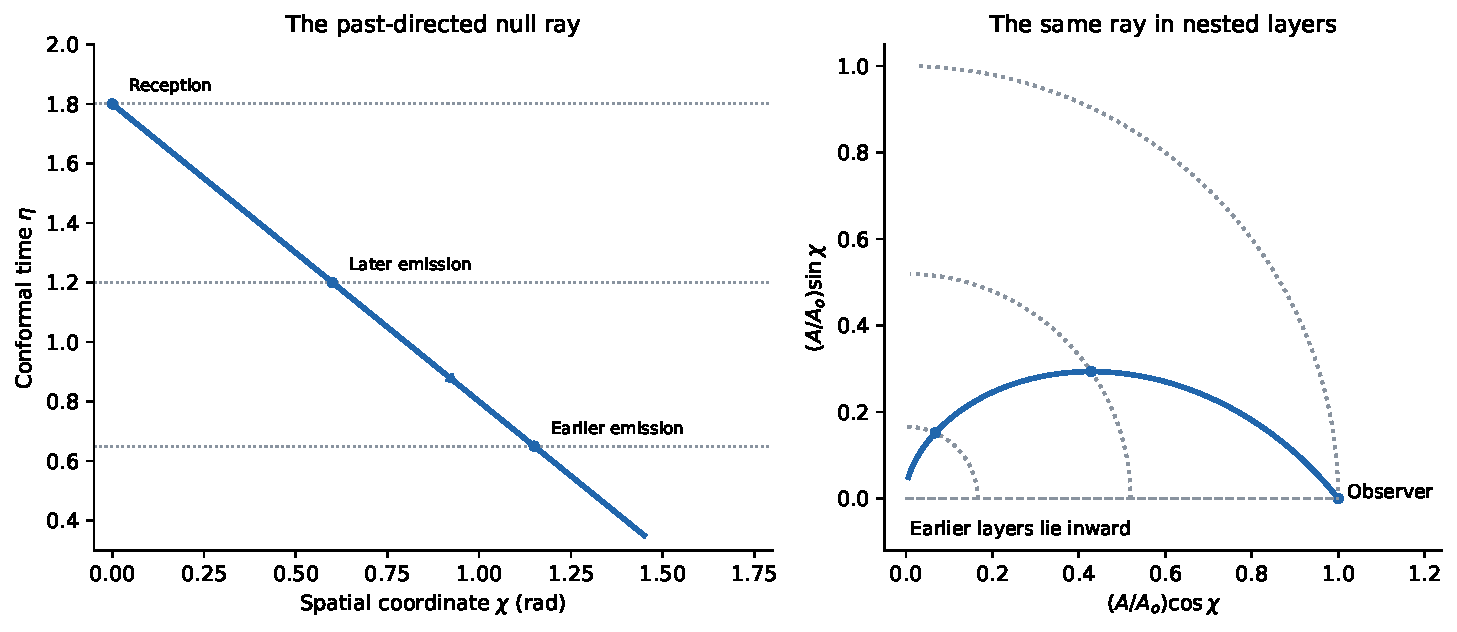
\includegraphics[width=\linewidth]{01-view-lines.pdf}
 \caption{The same closed-dust radial null ray in conformal and
 temporal--radial coordinates. Dotted curves mark corresponding times.
 Radius on the right encodes $A/A_o$; the observer is on the outer layer.
 The formal small-radius limit is not a location on any spatial slice.}
 \label{fig:baseline}
\end{figure}
\FloatBarrier
